%!TEX root = ../slides.tex
\section{ПЭТ - исследование}
\begin{frame}
    \frametitle{ПЭТ - исследование}
    \begin{itemize}
        \item Позитронно-эмиссионная томография (ПЭТ) — технология 
        визуализации, основанная на количественной и качественной 
        оценке биохимических процессов, происходящих в тканях \textit{in vivo}.
    \end{itemize}
\end{frame}
\subsection{Принцип работы ПЭТ}
\begin{frame}
    \frametitle{Принцип работы ПЭТ}
    \begin{figure}
        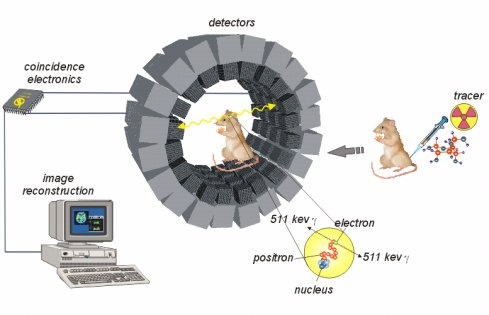
\includegraphics[scale=0.5]{pet.jpg}
    \end{figure}

    \begin{itemize}
        \item Как отличить здоровую ткань от «нездоровой»?
    \end{itemize}
    \[SUV_{\chi}=\frac{C(t)}{D/\chi}\]
\end{frame}


\begin{frame}
    \frametitle{Примеры ПЭТ - изображений}

    \begin{figure}[htbp]
        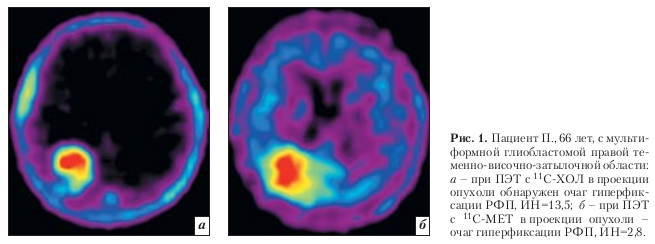
\includegraphics[scale=0.3]{pet_ex1.png}
        \hfill
        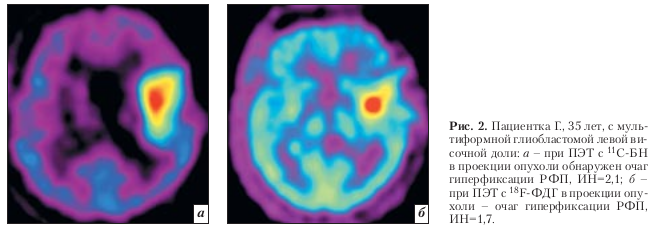
\includegraphics[scale=0.3]{pet_ex2.png}   
    \end{figure}

    \begin{figure}
        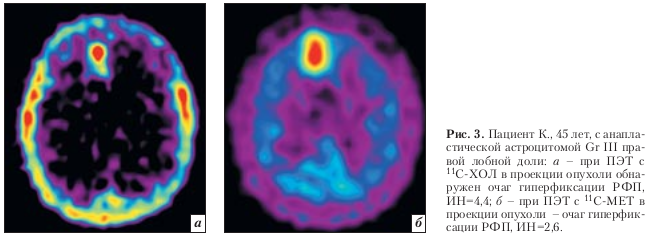
\includegraphics[scale=0.3]{pet_ex3.png}
    \end{figure}
\end{frame}

\subsection{ПЭТ/КТ, ПЭТ/МРТ}
\begin{frame}
    \frametitle{КТ, МРТ}
    \begin{itemize}
        \item Компьютерная томография (КТ) - это специальный метод визуализации, в котором используется рентгеновское излучение. 
        \item Магнитно-резонансная томография (МРТ) - метод визуализации, основанный на резонансе атомов водорода в организме человека на магнитное поле, 
        создаваемое томографом.
    \end{itemize}
    \begin{figure}[htbp]
        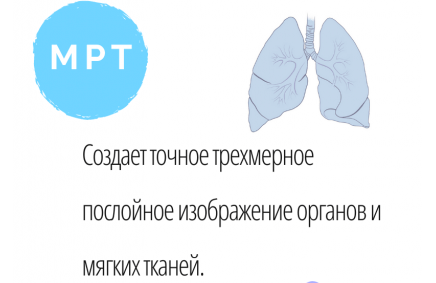
\includegraphics[scale=0.35]{mri.png}
        \hfill
        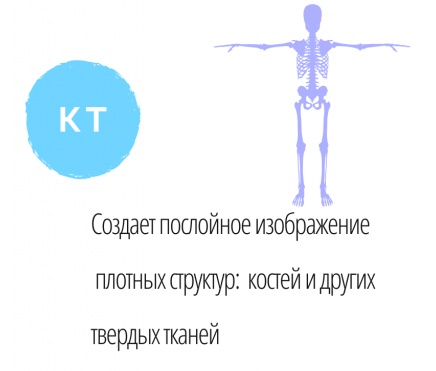
\includegraphics[scale=0.35]{ct.png}
    \end{figure}
\end{frame}

\begin{frame}
    \frametitle{ПЭТ/КТ, ПЭТ/МРТ}
    \begin{figure}
        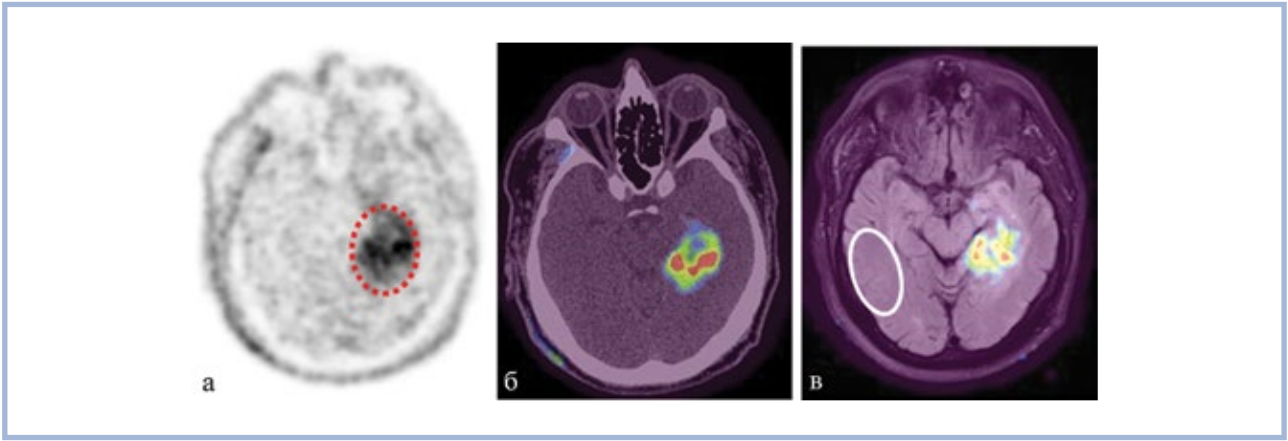
\includegraphics[scale=0.3]{pet_mri_ct.png}
    \end{figure}
\end{frame}